\chapter{The Adapter Framework}

\section{Introduction}

Changing requirements force software systems to include new components to extend their features. 
Software components are self-contained entities with a well-defined interface and behavior. 
For two components to function together they must be \emph{integrated} through a compatible interface. 
Typically such compatibility is not a given and it should be, often manually, established through additional programming. 
The integration task also entails binding the data values, i.e creating dependencies between the components. 
Once the data is represented through a compatible interface it is assigned to a target field and kept synchronized with the source data, this operation is called data binding.

The problem of incompatible interfaces is a common software engineering problem and its solution is captured in the \emph{adapter pattern} (cite Gamma). 
An adapter is a level of indirection between the incompatible interfaces, using one interface as the adaptee and the other as the target.  
This means the when an object of the target interface is expected but a source object of another interface is offered, the adapter which wraps the source object and implements the target interface is initialized. 

There are some issues attached to the traditional adapter pattern.
Firstly, its implementation can be problematic with some programming languages.
If we look at a class adapter, we see that it should be implemented with a language that allows multiple inheritance. 
Single inheritance programming languages like Java needs to use workarounds to achieve the same effect.
The implementation of object adapter pattern is more flexible, since it only needs to inherit from the target type. 
However this implementation also does not allow a single object adapter to adapt to multiple target types. 
A second point is that the adapter pattern adds a level of indirection between the source and the target, which needs to be maintained. 
Another drawback comes from the additional dependencies introduced by the adapter classes. 
The integration code has to refer to the specific adapter classes to initialize the desired objects. 
This has two side effects, first the implementation contains a direct reference to the adapter type instead of just the source and the target types. This introduces an additional maintenance efforts. 
Secondly the user is required to know exactly which adapter is responsible for a specific interface conversion.
Adapters are not a well-documented part of  a software.
Usually this information is communicated through a particular adapters name or one has to go inside that adapter class to understand the expected source and the target types. 
This process is error-prone as well as time consuming.

Adaptation is only one part of the integration problem. 
The second part entails establishing dependencies between the integrated components. i.e binding. 
In component-based design loose-coupling is an important principle.  
Dependency injection (DI) (cite fowler) is a lightweight method for keeping modules loosely coupled by delegating the creation of concrete objects to so-called \emph{injectors}. 
This approach allows a customizable and a decoupled way of creating dependencies, while maintaining loose coupling.

Typically these two parts, adaptation and binding, are handled separately from each other during integration. 
We think these parts can be unified from the users perspective by providing a concise interface for the whole integration task.
In order to achieve this goal we have designed the \zamk framework, which unites dependency injection with \emph{under-the-hood} adaptation logic.
For our framework we have decomposed the traditional adapter pattern and created \emph{converters}, which are user-defined inheritance-free classes. 
\zamk comes with its own dependency injection mechanism that is used with a designated domain-specific language called \gluer. 
The dependency injection logic is intertwined with the adaptation logic which uses the converter registry to perform automated adaptation between source and target types. 
We automate the adaptation process by exploiting the type hierarchies and provide checks and context-relevant messages for correct integration. The details of the framework will explained throughout the chapter.

\section{Motivation}
\label{sec:adapter:motiv}

We have mentioned some problems attached to the traditional adapter pattern\footnote{Throughout this chapter, the term adapter pattern will refer to the object adapter pattern. The class adapter pattern will explicitly include the term class.}. Let us give an example which illustrates these problems in a detailed manner. 
We assume we have a plot drawing software which uses the Cartesian coordinate system to represent the points in the plot. 
The software includes a data component which contains a class called \lstinln{Cartesian} which includes two fields \lstinln{x, y}, that represents the values on the x-axis and y-axis respectively. 
This class also includes getters and setters for these fields (\lstinln{Component1} in Figure~\ref{fig:components}).
A new requirement is received which states that the software must also support polar coordinates, and the points on a plot should be shown in a selected format (Cartesian or polar). 

In order to support polar coordinates, a new component which contains classes to represent such data is introduced (\lstinln{Component2} in Figure~\ref{fig:components}). The class \lstinln{Polar} contains two field \lstinln{r} representing the radius and \lstinln{theta} of type \lstinln{Angle}. This component is to be integrated with the \lstinln{Cartesian} component. It should be possible to obtain the \lstinln{Polar} representation of any \lstinln{Cartesian} object by using an \emph{adapter}.

\begin{figure}
\centering
\begin{tikzpicture}[scale=0.7, transform shape]

\begin{umlpackage}[x = 0, y = 0]{Component1}

\umlclass{Cartesian}
{
	x: double \\
	y: double \\
}
{
	
}

\end{umlpackage}

\begin{umlpackage}[x = 6, y = 0]{Component2}

\umlclass[x = 0, y= 0]{Polar}
{
	r: double \\
	theta: Angle \\
}
{
	
}

\umlclass[x = 4, y= 0]{Angle}
{
	value: double
}
{
	+getSin() : double \\
	+getCos() : double
}

\end{umlpackage}



\end{tikzpicture}
\label{fig:components}
\caption{UML diagram for the two components}
\end{figure}

An abstract view of the traditional object adapter pattern is shown in Figure~\ref{fig:oapattern}. The adapter pattern relies on inheritance and adds a level of indirection between the \lstinln{Client} and the \lstinln{Target}. The application of this pattern to the example case requires creating a Cartesian to polar adapter (\lstinln{Cartesian2PolarAdapter}) which takes a \lstinln{Cartesian} object as an \emph{adaptee} and extends the \lstinln{Polar} class to override its methods (Figure~\ref{fig:objadapter}). An implementation for this adapter is given in listing~\ref{lst:objadapterlst}.


\newsavebox{\cartesiantopolar}
\begin{lrbox}{\cartesiantopolar}
\begin{lstlisting}
public class Cartesian2PolarAdapter extends Polar{
	Cartesian adaptee;
	public Cartesian2PolarAdapter(Cartesian c) {
		this.adaptee = c;
	}
	public double getR()
	{
		return Math.sqrt(Math.pow(adaptee.getX(), 2) + Math.pow(adaptee.getY(), 2)));
	}
	public Angle getTheta()
	{
		return new Angle(Math.atan(adaptee.getY()/adaptee.getX())));
	}
}
	\end{lstlisting}
\end{lrbox}

\newsavebox{\cartesiantopolaraop}
\begin{lrbox}{\cartesiantopolaraop}
\begin{lstlisting}
public aspect Cartesian2PolarAdapter {

	declare parents: Cartesian extends Polar; ~\label{lst:line:it}~

	public double Cartesian.getR()
	{
		return Math.sqrt(Math.pow(this.getX(), 2) + Math.pow(this.getY(), 2));
	}
	
	public Angle Cartesian.getTheta()
	{
		return new Angle(Math.atan(this.getY()/this.getX()));
	}
}

	\end{lstlisting}
\end{lrbox}


\begin{figure}
\centering
\subfloat[Abstract view of the object adapter pattern]{

\begin{tikzpicture}[scale=0.5, transform shape]

\umlemptyclass{Client}
\umlclass[x = 4, y = 0]{Target}{ 
 
  }{ 
  + Request()
} 

\umlclass[x = 8, y = 0]{Adaptee}{ 
 
  }{ 
  + SpecificRequest()
}


\umlclass[x = 6, y = -3]{Adapter}{ 
  +adaptee : Adaptee
  }{
  + Request()
}

\umlinherit{Adapter}{Target}
\umluniassoc{Client}{Target} 
\umlaggreg{Adapter}{Adaptee}

  \end{tikzpicture}

\label{fig:oapattern}
}
\hfill
\subfloat[Concrete view of the object adapter for the example case]{
\begin{tikzpicture}[scale=0.5, transform shape]

\umlemptyclass{Client}
\umlclass[x = 4, y = 0]{Polar}{ 
 
  }{ 
  + getR() \\
  + getTheta()
} 

\umlclass[x = 8, y = 0]{Cartesian}{ 
 
  }{ 
  + getX() \\
  + getY()
}


\umlclass[x = 6, y = -3]{Cartesian2PolarAdapter}{ 
  +adaptee : Cartesian
  }{
  + getR() \\
  + getTheta()
}

\umlinherit{Cartesian2PolarAdapter}{Polar}
\umluniassoc{Client}{Polar} 
\umlaggreg{Cartesian2PolarAdapter}{Cartesian}

  \end{tikzpicture}

\label{fig:objadapter}
}
\vfill
\subfloat[The implementation for the \lstinln{Cartesian2PolarAdapter}]
{\usebox{\cartesiantopolar}
\label{lst:objadapterlst}}
\caption{The diagram of the object adapter and the corresponding Java implementation}
\end{figure}

In their paper on aspect-oriented implementation of gang-of-four design patters (\cite{hannemann:oopsla02}) Hannemann and Kiczales mention an adapter pattern implementation using inter-type declarations. 
According to the auxiliary code they provide with this study, they propose the adaptee class should subclass the target class, which results as the diagram shown in Figure~\ref{fig:hkaop}. For our example case the \lstinln{Cartesian} class will directly have to subclass the \lstinln{Polar} class and implement its method using its \lstinln{x, y} field values. This is depicted in the aspect shown in Listing~\ref{lst:objadapteraoplst}. The inter-type declaration on line~\ref{lst:line:it} declares the inheritance relation and the subsequent method implementations are woven into the \lstinln{Cartesian} class.

\begin{figure}
\centering
\subfloat[Abstract view of the object adapter pattern with inter-type declarations]{
\begin{tikzpicture}[scale=0.6, transform shape]
\umlemptyclass{Client}
\umlclass[x = 4, y = 0]{Target}{ 
 
  }{ 
  + Request()
} 

\umlclass[x = 4, y = -3]{Adaptee}{ 
  }{ 
  + SpecificRequest() \\
  + Request() 
}
\umlinherit{Adaptee}{Target}
\umluniassoc{Client}{Target} 
\end{tikzpicture}
\label{fig:hkaop}
}
\hspace{20pt}
\subfloat[Concrete view of the aspect-oriented adapter pattern for the example case]{
\begin{tikzpicture}[scale=0.6, transform shape]
\umlemptyclass{Client}
\umlclass[x = 4, y = 0]{Polar}{ 
 
  }{ 
  + getR() \\
  + getTheta()
} 

\umlclass[x = 4, y = -3]{Cartesian}{ 
  }{ 
  + getX() \\
  + getY() \\
  + getR() \\
  + getTheta 
}
\umlinherit{Cartesian}{Polar}
\umluniassoc{Client}{Polar} 
\end{tikzpicture}
\label{fig:hkaopex}
}
\vfill
\subfloat[The implementation for the \lstinln{Cartesian2PolarAdapter} in AspectJ]
{\usebox{\cartesiantopolaraop}
\label{lst:objadapteraoplst}}
\caption{The diagram of the object adapter and the corresponding Java implementation}
\end{figure}

The obvious problem with this implementation is that it would quickly become unusable due to Java's single inheritance. 
If the \lstinln{Cartesian} class were extending any other class, that it would not be possible to declare that it also extends \lstinln{Polar} class. 
Also such a declaration means that a \lstinln{Cartesian} object is also a \lstinln{Polar} object, which is prone to create ambiguities in an object-oriented setting. 

In order to integrate the polar coordinates into our plotting software, we need to alter some code. 
According to the selection made in the GUI, the information box should display the coordinate value in the correct format. 
An hypothetical example for the integration code is given in Listing~\ref{lst:integration}.
On line~\ref{lst:integration:adapt} we see an explicit reference to the class \lstinln{Cartesian2PolarAdapter}.
In this simple example, this reference is manageable. 
However if several such extensions are to be made, there will be several such references.
This requires keeping track of all referenced classes; if one is deleted then we would have errors in our code, due to broken dependencies. 
Also the user performing the integration has to know all the specific classes that are responsible for adaptations; depending solely on naming is error-prone. 
This slows down the integration process.

\begin{lstlisting}[float, caption={The integration of Polar coordinates}, label={lst:integration}]

public void viewPointValue(Point selected)
{
	if(GUI.format == CARTESIAN)
		GUI.createNewValueBox(selected.loc(), selected.getCoordinates().toString());
	else if(GUI.format == POLAR)
	{
		Polar p = new Cartesian2PolarAdapter(selected.getCoordinates()); ~\label{lst:integration:adapt}~
		GUI.createNewValueBox(selected.loc(), p.toString());
	}
}
\end{lstlisting}

We have used the plotter example to illustrate some of the issues related to the traditional adapter pattern and component integration using these adapters.
Our goal is to provide a solution to the these issues in the form of a framework. 
Our framework has the following requirements:

\begin{easylist}[enumerate]                                          
\ListProperties(Style2*=,Numbers=a,Numbers1=R,FinalMark=.)
& Use adapters without creating dependencies to specific adapter classes.
& Means to separate the adaptation logic from the integration logic during development time.
& Inheritance-free adapter structures. 
& Adapters are found automatically given a source object and a target type.
& Dependency injection based binding via a declarative language that works with the adaptation logic.
\end{easylist}

\section{Approach}
We have concluded with a set of requirements in Section~\ref{sec:adapter:motiv}. In this section we will explain the details of the \zamk framework which is designed according to these requirements. 

\zamk is a development framework specifically tailored for adapter-based integration. 
It offers a new and a light-weight way of defining adapters; these light-weight structures are called \emph{converters}. 
Converters are user-defined classes that are free of inheritance and they are stateless. 
\zamk runtime is responsible for finding the correct converter, given a source and a target object. 
This means the only additional dependency we have to include in the implementation is the \zamk runtime API. 
Since the user doesn't have to refer to specific adapters, \zamk allows separation of adaptation and binding concerns during integration.
\zamk also comes with its own binding language, so-called \gluer, which uses dependency injection under-the-hood. 
\gluer~ is a domain-specific language and its declarative nature allows compile-time checks.
The user is flexible in how she chooses to use \zamk, she can either use the \gluer language or she can call the runtime API directly. 
Integration using \zamk also helps separating the binding concern and the adaptation concern from each other.  

\begin{figure}
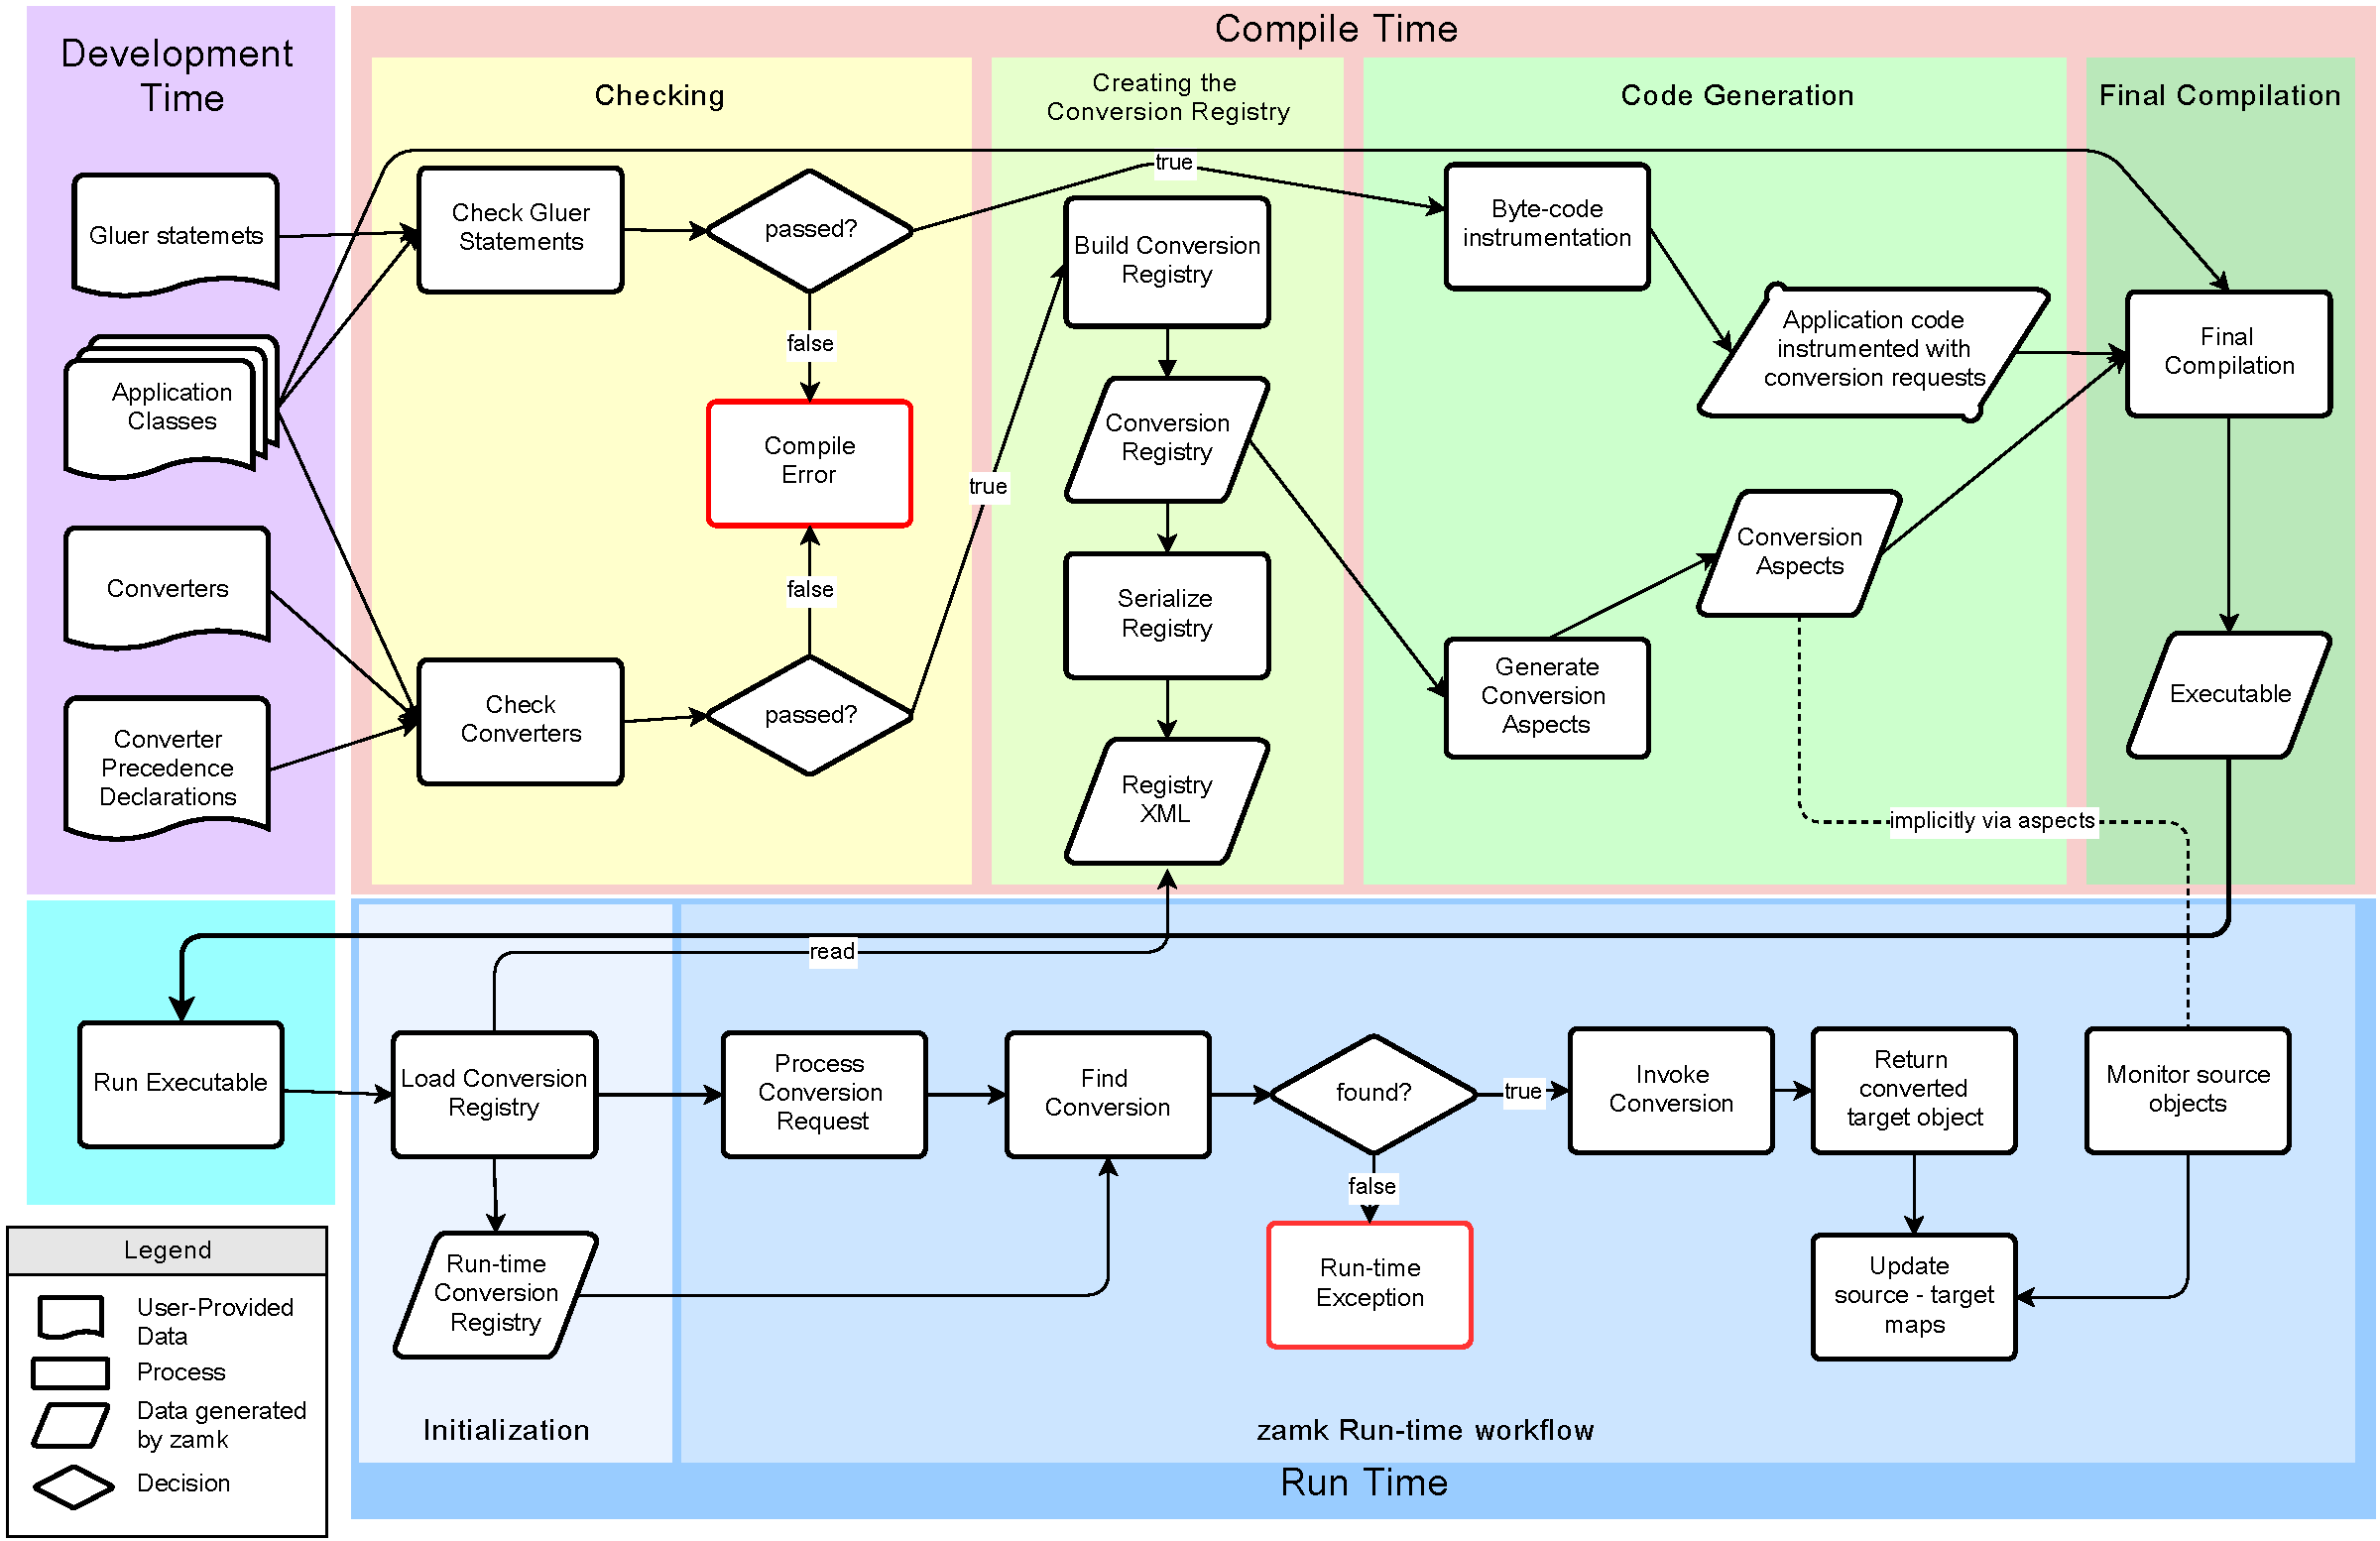
\includegraphics[height=\textwidth, angle=90]{chapteradapters/bigpicture.pdf}
\caption{An overview of the \zamk framework}
\label{fig:framework}
\end{figure}

In Figure~\ref{fig:framework} shown an overview of the stages that are necessary to perform an integration using \zamk.
\zamk requires user-defined input to perform an integration.
This input is created during \emph{development time} and includes the converters, gluer files that contain the gluer statements, converter precedence declarations and the classes of the applications that will be integrated. 

Once this input is provided, the \zamk compiler work-flow starts. This work-flow is composed of the following operations, which are performed sequentially.

\begin{easylist}[enumerate]
& Checking: There are two checkers which are responsible for checking the \gluer files and converter classes. The gluer checker performs the syntax checking; it also checks if the references made in the \gluer statement actually exist in the application code. The converter checker performs type checking and well-formedness checking. If any of these checks fails, a compile-error is produces. 
&  Conversion registry: When the converter checking is finished without any problems, \zamk creates a conversion registry (one converter may include multiple conversions), which is serialized in XML format.
& Code Generation: This step consists of two separate generation processes. Byte-code instrumentation is responsible for inserting \zamk conversion requests to the places indicated as the binding points defined in the \gluer statements. The converter registry created in the previous step is used to generate the conversion aspects, which are responsible for book-keeping the already converted objects. 
\end{easylist}
 
When the compile-time work flow is complete a final compilation step is performed, which makes sure the instrumented application classes and the generated files do not contain any errors. 
At the end of this step we obtain a \zamk run-time ready code, in this figure we assume the final compilation product is an executable.

The \zamk run-time starts with an initialization step, which loads the conversion registry that is serialized during runtime. 
The loading process produces a data structure called run-time conversion registry, which is used by the run-time work flow to locate conversions.
The compiled program contains \zamk conversion requests which trigger the conversion finder. 
A conversion request contains the source object and the desired target type to which the source object should be converted. 
The \emph{find conversion} process searches for the correct conversion by using the type information included in the conversion request. 
If a suitable conversion cannot be found, \zamk produces a run-time exception indicating the error. 
If a conversion is found, one of two things can happen. Either the request may result in a new conversion, i.e. it may trigger the process to create a new source--target pair. In order to create a new source--target pair, the corresponding conversion method is invoked and the newly created target object is returned. 
The conversion aspects are responsible for monitoring the source objects which are associated with a target object. Or \zamk may find that a request to the same target type was processed before with the given source object. In that case the existing target object is retrieved and returned. 







\subsection{Decomposition of the adapter pattern}
% In order to overcome the issues caused by the implementation of the traditional adapter pattern, we have decomposed it to offer a more concise way of implementation. 
% ``How much should an adapter do?'' is a common question developers ask when implementing adapters. 
% The answer is ``It should do how much it has to in order to adapt''. 
% % The ``how much'' depends on how many methods
In the traditional adapter pattern, the adapter class has an adaptee; if this adaptee's value is changed, it directly effects the return values of the method in the adapter's interface.
We have decided to decompose adaptation as a one-time conversion and a series of updates during an objects life-cycle. 
Our decomposed adapter pattern consists of two parts, first is a class that has two methods, a convert and an update method. 
The second part is an \emph{aspect} which contains a hash-map of source(adaptee) and target objects. 
The responsibility of this aspect is to monitor the source (adaptee) objects and update the target objects if a source object changes.

In Figure~\ref{fig:conv1} the first step of the adaptation process is shown. 
A new adaptation requested by giving a source object and a target type. 
In the traditional adapter pattern this source object is the adaptee and an adapter which is a subtype of the target type is instantiated that aggregates this source object. 
In our adaptation process this source object is passed onto the convert method of an appropriate converter (automatically found by the framework, section~\ref{sec:adapter:find}) and this method returns the corresponding target object, which is initialized according to the values provided by the source object. 
When a new target object is created, the \zamk runtime registers the source-target tuple in a hashmap. 
This hashmap replaces the \emph{has-a} relationship between the adapter and the adaptee. 


Once a target object is linked to a source object, they are kept synchronized. 
This is ensured by the monitor aspect. 
This aspect monitors the events which change the source objects, when such an event is encountered it retrieves the corresponding target object. 
Then it triggers the \emph{update} method in the converter class to update the target object that is linked to the changed source object.

\begin{figure}
\subfloat[A new adaptation request]{
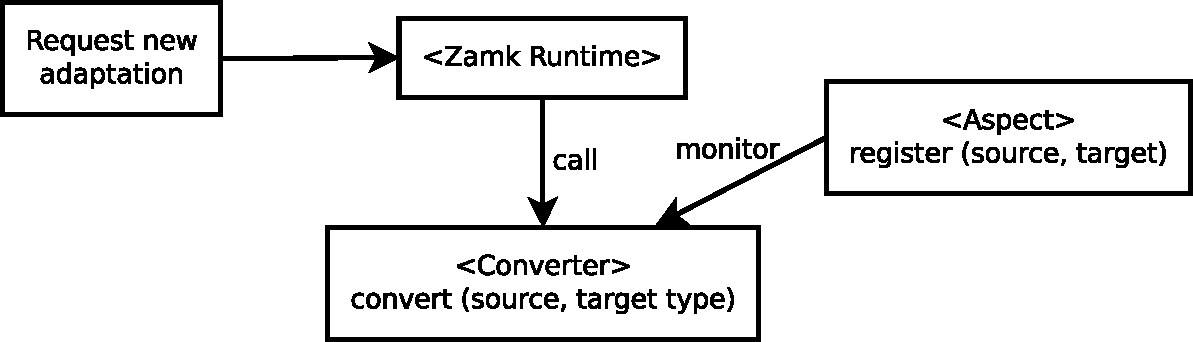
\includegraphics[width=0.45\textwidth]{chapteradapters/conv1.pdf}
\label{fig:conv1}
}
\subfloat[Keeping source and target objects synchronized]{
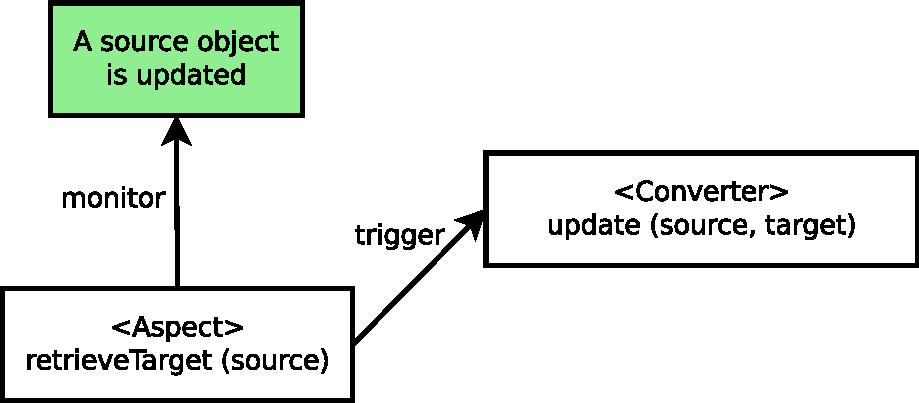
\includegraphics[width=0.45\textwidth]{chapteradapters/conv2.pdf}
\label{fig:conv2}
}
\end{figure}

In this method of adaptation, there's no need to create an intermediate adapter type.
The converter directly creates an object of the target type and keeps it up-to-date. 
As we will explain in section~\ref{sec:adapter:compile}, the user only has to define the converter class. 
The monitor aspect is generated during compile-time by \zamk framework. 
%Our decomposition provides a uniform way of implementing adapters.


\subsection{Compile-time}
\label{sec:adapter:compile}

In this section we will explain the elements and modules that are involved during the compile-time of the framework. In figure~\ref{fig:ctwf} a compile-time work-flow is shown. The user is responsible with providing converters that are specific to her application. The converters are required to adhere to a specific structure, which is discussed in section~\ref{sec:adapter:converter}. 
If \zamk's built-in dependency injection module is to be used, then the user should also provide a \gluer~file that includes the necessary \gluer~statements. 

All of the provided input is then checked by \zamk's compile-time checker. If any problems are found, then this is reported as a compile error or a warning. When the checking is passed without any problems \zamk's code-generator is invoked. \gluer~ files are processed by the byte-code generator, which performs \emph{weaving} of the dependencies to the target components. The converters are processed by the aspect-generator which generated the monitoring and management aspect for each converter, concluding the compile-time work-flow of \zamk.
\begin{figure}
\centering
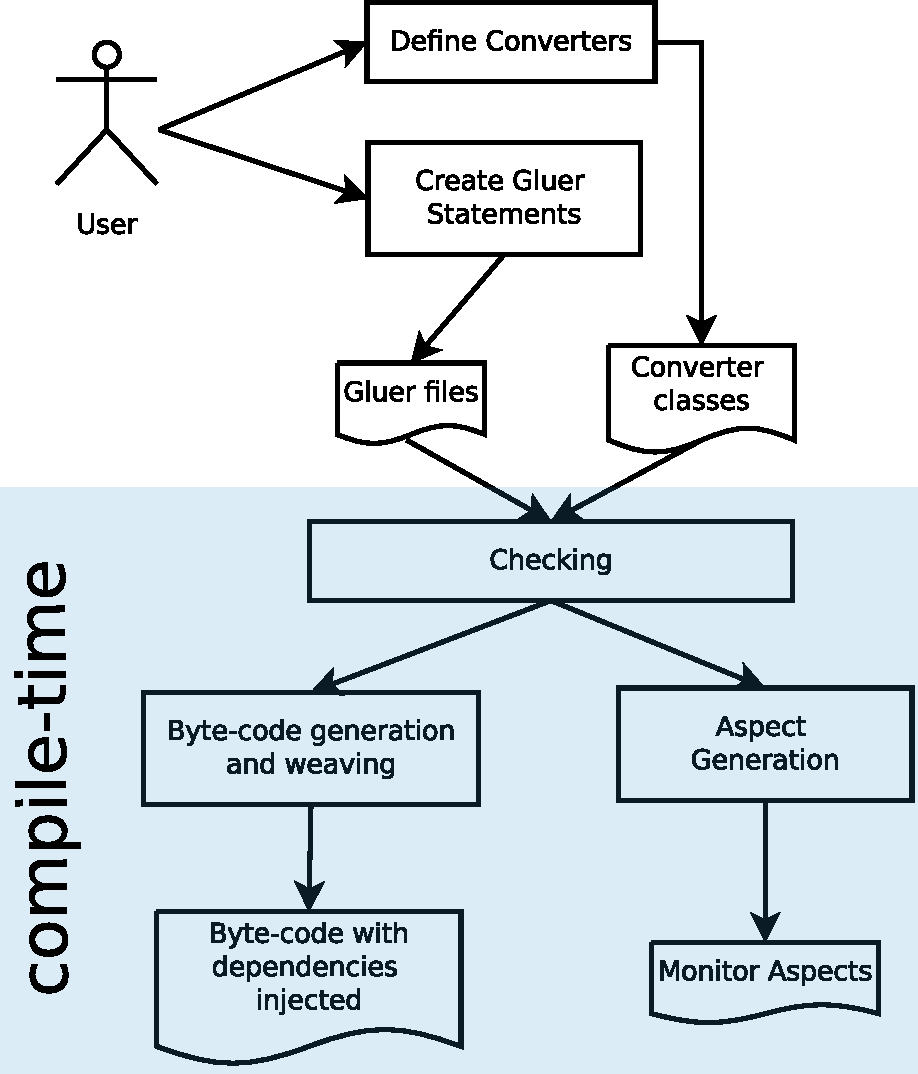
\includegraphics[width=0.45\textwidth]{chapteradapters/ctv.pdf}
\caption{The user provided input and the compile-time workflow of \zamk}
\label{fig:ctwf}
\end{figure}

\subsubsection{Gluer DSL}
The \gluer~ language is a concise DSL that is designed to declare dependencies between fields and objects. 
We have developed the \gluer~ language to offer an external, non-intrusive way of declaring bindings. 
Essentially the \gluer~ is an external dependency injection declaration which creates the objects to be injected, but is connected to an adaptation logic which can process the created objects before injection.
Therefore the \gluer~ is not a plain dependency injection language. 
This is why we chose the keyword \lstinln{glue} instead of \lstinln{inject}. 

A simple gluer statement looks like the following:

\lstinline~glue field <target-field> with <source-class> [using <converter>]~

\begin{description}
\item[<target-field>] The target field is a fully qualified name of a non-static field of a class. 
It can refer to any type, including primitive types. 
\end{description}

\begin{description}
\item[<source-class>] The source class represents the class to be instantiated and injected to the target field. There are several options for creating this objects.
	\begin{description}
	\item[new] The \lstinline{new} statement is followed by a fully classified name of a class. This means, whenever an object is to be injected, it should be newly created using the \emph{default constructor} of the source class. 

	\item[single] Similar to \lstinline{new}, \lstinline{single} statement is followed by a fully qualified name of a class, which is instantiated when an injection is triggered. The difference is instead of creating a new object each time, a \emph{single} object is reused among injections.
	\TODO{possible use case}

	\item[retval] Short for ``return value'', this keyword is followed by a fully qualified reference to a method, which returns the object we would like to inject. When an injection is triggered, the method is called and the returned value is glued to the injection field.
	\end{description}
\item[using keyword] The \lstinln{using} keyword is optional and can be used to override the automated converter finding logic. With this keyword the user can point to a specific converter to be used while converting the source object to the target type, before the injection. 
\end{description}

\paragraph{Checks} \gluer~also allows us to perform some compile-time checks to ensure the correctness of the \lstinln{glue} statements. 
All of these checks result in compile errors that contain specific information about the place and the cause of the error.

\begin{itemize}
\item Target-field is checked to see if it actually exists.
\item For creating the source object with the \lstinln{new} and \lstinln{single} keywords, the framework requires that the source class contains a no-argument constructor. For the \lstinln{retval} keyword, the framework checks if the referred method exists.
\item The \lstinln{using} keyword triggers two checks. First one checks if the referred converter exists and the second one checks if the converter is suitable for converting from the source class to the target field. 
\item If the \gluer~statements are error free up to this point, then a conflict check is performed to see if any two \gluer~ statements try to inject into the same field. 
\end{itemize}



\subsubsection{User-defined Converters}
\label{sec:adapter:converter}
The users of \zamk are responsible for creating a converter, which we classify as a domain-specific aspect. Although the user creates a class, it adheres to a specific structure and it is annotated order to be managed as part of an aspect. 

A converter has three important requirements:
\begin{enumerate}
\item It should be annotated with the \lstinln{@Converter} annotation
\item It has to include at least two \emph{static} methods:
	\begin{enumerate}
	\item A \emph{convert} method that is annotated with \lstinln{@Convert}. This method takes a single parameter and cannot be void. 
	\item An \emph{update} method that is annotated with \lstinln{@Update}. This method takes two parameters of the same type and is void.
	\end{enumerate}
\item There cannot be two convert methods that has the same argument and return types in a single converter. Same is true for the update method.  
\end{enumerate}

The convert method contains the logic for converting a source object to a target object. It takes a source object as its single argument and returns the corresponding target object. The update method contains the logic for updating a target object. It takes two arguments of the type target; the first represent the old value of the object and the second the updated value. Inside the method the second argument is used to update the first argument. 

Referring back to our example given in section~\ref{sec:adapter:motiv}, a user-defined adapter for the \lstinln{Cartesian-Polar} conversion that conforms to the requirements above can be defined as shown in listing~\ref{lst:c2pconverter}. In this example we have defined two methods; \lstinln{cart2polar} which is annotated as the convert method takes a source object of type \lstinln{Cartesian} and returns a \lstinln{Polar} object, the values of which is calculated using the source object. The second method is \lstinln{updatePolar}, which updates the \lstinln{old} \lstinln{Polar} object using the field values of the \lstinln{newValue Polar} object. Note that since the methods are annotated there are no restrictions on the method naming. 

\begin{lstlisting}[float, caption={A converter defined for converting a Cartesian object to a Polar object}, label={lst:c2pconverter}]
@Converter
public class Cartesian2PolarUser{
	@Convert
	public static Polar cart2polar(Cartesian source)
	{
		//calculations
		return new Polar(..));
	}
	@Update
	public static void updatePolar(Polar old, Polar newValue)
	{
		old.r = newValue.r;
		old.the = newValue.the;
	}
}
\end{lstlisting}

This converter can also include methods which convert from \lstinln{TypeA} to \lstinln{TypeB} following the same rules. The \lstinln{@Converter} annotation simply marks a class to be found by \zamk. When \zamk finds a converter class, it expects that it has one or multiple \emph{pairs} of convert and update methods. If a convert methods is found to be without an update methods or vice versa, this results in a compile error. The convert-update method pairs should be declared in the same converter. \zamk does not merge methods from separate converter classes. 

If the developer declares another pair of convert-update methods in the same converter which is the inverse of the previously declared one, this conversion is registered as a \emph{two-way} conversion. 
For example if we add the convert and update methods for \lstinln{Polar} to \lstinln{Cartesian} conversion to the converter in listing~
\ref{lst:c2pconverter} then \zamk will register a two way conversion between these types.
From the developer's perspective implementation requirements do not change, \zamk handles the operations required to keep converted objects synchronized.


When a pair of convert and update method are found, some type checks are performed. In order to register a conversion \zamk looks a the convert method's source (single parameter) and target (return) types. The accompanying update method \emph{must} take arguments of exactly the target type. Otherwise a compile error indicating the situation is given to the user. 

Converters do not need to use inheritance to perform adaptations.
Since all the adaptation related methods are static, they do not need to be initialized to function; they are stateless.
Their well-structured definition allows the developer to implement only what is necessary to perform an adaptation. 
Converters are concise and light-weight structures that encapsulate the adaptation concern.

\subsubsection{Conversion Registry}
\label{sec:adapter:convreg}
During compile-time a converter registry is created and serialized using the annotated converter classes. 
The procedure for creating the converter registry can be seen in Procedure~\ref{alg:convreg}. 

\begin{algorithm}
\caption{Creating the conversion registry}\label{alg:convreg}
	\begin{algorithmic}[1]
		\Procedure{createRegistry}{}
			\State $converters \gets $ all classes annotated with @Converter
			\ForAll{$c \in converters$}
			\State $cMethods \gets $ all methods in $c$ annotated with @Convert
			\State $uMethods \gets$ all methods in $c$ annotated with @Update
			\ForAll {$cm \in cMethods$}
			\State $sourceType \gets $ the argument type of $cm$
			\State $targetType \gets $ the return type of the $cm$
			\ForAll{$um \in uMethods$}
				\If{$um.argumentType = targetType$}
					\State $conversion \gets (sourceType, targetType, cm, um)$
					\State add $conversion$ to $record$
					\State remove $cm$ from $cMethods$
					\State remove $um$ from $uMethods$
				\EndIf
			\EndFor
			\EndFor
			\State registerTwoWayConversions(record)
			\State add $(c.FQN, record)$ to $registry$
			\EndFor
			\State serialize($registry$)
		\EndProcedure
	\end{algorithmic}
\end{algorithm}


This procedure assumes the converter class is structurally correct, i.e. the methods are properly annotated and there is exactly one matching update method for each convert method in a converter. 
The createRegistry procedure first finds all classes annotated with \lstinln{@Converter}. 
From each converter class it find the convert and update methods and puts them into separate lists. 
For each convert method found in the converter the variables $targetType$ (the return type of the convert method) and $sourceType$ (the argument type of the convert method) are initialized. 
Then the matching update method is found by iterating over the list of update methods and comparing their argument the target types. 
When an update method is found and then the record of the conversion is created. 

The $record$ data structure contains the list of $conversion$ items a converter contains. A $conversion$ consists of the the source and the target types, the name of the convert and update methods. 
The convert and update methods included in the created $conversion$ are removed from the corresponding lists. 
When all conversions in a converter is found, the $record$ for a single converter class is complete. 
However at this point the $record$ does not contain any information about two-way converters.

The registerTwoWayConversions(shown in Procedure~\ref{alg:regtwoway}) procedure processes the $record$ list and changes its contents if it contains any two-way conversions.
This procedure iterates over the conversion list $record$ and tries to find conversions which have the inverse source and target types. 
Once a pair of such conversions are found, a $newConversion$ which contains the source and the target types and the convert and update method names of both conversions is created. 
The $newConversion$ items are collected in a separate list called $newRecord$ and the individual conversions forming a two-way conversion are marked in the $record$ list. 
After all two-way conversions are found, the marked entries from $record$ are removed and the new entries collected in $newRecord$ are added to list $record$. 
This procedure is also responsible for assigning the unique IDs to each conversion, which is done in the for loop shown on line~\ref{alg:idloop}.
This unique ID is later used in the aspect generation as the aspect unique ID. 
Once the $record$ list is in its final form it is mapped to the $registry$with the converter's fully-qualified name as the key. 
After the list of converters is exhausted the $registry$ is fully populated.
The last operation is the serialization of the $registry$ to an XML file, which is done by the serialize operation at the end of the procedure.

\begin{algorithm}
\caption{Finding the two-way conversions}\label{alg:reg2way}
	\begin{algorithmic}[1]
		\Procedure{registerTwoWayConversions}{$record$}
		\ForAll{unmarked $x \in record$}
		\ForAll{unmarked $y \in record$}
			\If{$y.sourceType = x.targetType$}
				\If{$y.targetType = x.sourceType$}
				\State $newConversion \gets (sourceType, targetType, x.convert,$
				\\\hspace{\algorithmicindent}$ x.update, y.convert, y.update)$
				\State mark $x$ and $y$
				\State add $newConversion$ to $newRecord$
				\EndIf
			\EndIf
		\EndFor
		\EndFor
		\State remove marked conversions from $record$
		\State merge $newRecord$ and $record$
		\ForAll{$r \in record$} \label{alg:idloop}
		\State assign $uid$ to $r$
		\EndFor
		\EndProcedure
	\end{algorithmic}
\end{algorithm}

The registry is serialized as an XML file, with the format shown in Listing~\ref{lst:registry}. 
The XML structure adheres to the class structure; multiple conversion tags are enclosed with a converter tag, which takes the fully-qualified name of the converter as a value. 
The conversion tag marks if the conversion is a two way conversion and contain the source--target types for the conversion, and the convert--update method pair for each conversion direction (source-to-target and target-to-source). 
The convert and update tags contain the method names for convert and update methods respectively. The tags marked with \emph{1} are the methods responsible for the conversion from source-to-target, and following tags marked with \emph{2} are the convert and update methods for the inverse conversion, if the conversion is indeed a two way conversion. 

\begin{lstlisting}[float, language=XMLRegistry, caption={The XML code for a registry item}, label={lst:registry}]
<converter = [FQN]>
	<conversion uid=".." twoway = [true|false]>
		<source>[source-type]</source>
		<target>[target-type]</target>
		<convert = "1">[convert-method]</convert>
		<update = "1">[update-method]</update>
		<!--For two-way conversions-->
		<convert = "2">[convert-method 2]</convert>
		<update = "2">[update-method 2]</update>
	</conversion>
	<conversion...
</converter>
\end{lstlisting}


\subsubsection{Code Generation}

There are two separate code generation modules included in \zamk. The first one is the byte-code generation and weaving module which is used to generate code from \gluer~statements. 
The second one is the aspect generator, which uses user-defined converters to generate the monitoring and managing aspects, so-called conversion aspects, for each converter.

\paragraph{Byte-code generation and Weaving}
\TODO{get the details from Arnout}
Since \gluer~is a proof of concept implementation it only supports constructor injections. 
This is indicated by the \lstinln{field} keyword. 
It is also possible to extend the grammar and the byte-code generator to implement setter injections. 
\TODO{discuss}

\paragraph{Aspect Generator}
For each convert-update method pair in a user-defined converter a specialized aspect is generated. The template for this aspect is shown in listing~\ref{lst:genaspect}. 


\begin{lstlisting}[float, caption={The code generation template for producing an adaptation-specific aspect}, label={lst:genaspect}]
public privileged [name][source-type]2[target-type]GenAspect extends ZamkRuntime{
	private static aspectUID = [..]; ~\label{lst:genaspect:auid}~
	[name][source-type]2[target-type]GenAspect() ~\label{lst:genaspect:cons:b}~
	{
		ZamkRuntime.register(aspectUID, map);
	} ~\label{lst:genaspect:cons:e}~
	Map<[source-type], [target-type]> map = new WeakHashMap<[source-type], [target-type]>(); ~\label{lst:genaspect:map}~
	
	pointcut updateObserverThis(Object c): updateObserver(c) && if(c instanceof [source-type]); ~\label{lst:genaspect:uot}~
	after(Object c): updateObserverThis(c)
	{
		[source-type] obj = ([source-type])c;
		if(map.containsKey(obj)){
			[name].[update-method](map.get(obj), [name].[convert-method](obj)); ~\label{lst:genaspect:update}~
		}	
	}
}
\end{lstlisting}




Let us explain this template in detail. 
\lstinln{[name]} represents the user-defined converter's class name. We concatenate the the source and the target type names to create \lstinln{[source-type]2[target-type]} and \lstinln{GenAspect} at the end of \lstinln{[name]} to create the unique name for the generated aspect.
Since a single converter class can include multiple convert-update pairs, the aspect names also include the type information in their names.
Every generated aspect extends the abstract aspect \lstinln{ZamkRuntime}. 
The details of this aspect will be covered in section~\ref{sec:adapter:runtime}.

Each aspect has a unique ID called \lstinln{aspectUID} (line~\ref{lst:genaspect:auid}) and a constructor which is called create a \emph{singleton} instance of the aspect (lines~\ref{lst:genaspect:cons:b}--\ref{lst:genaspect:cons:e}). 
The \lstinln{aspectUID} is the conversion unique ID which is assigned during the generation of the conversion registry. 
Inside this constructor the aspect registers its \lstinline{map} to the \zamk runtime with its unique ID, which is used for storing the source--target pairs. The declaration of this \lstinln{map} is shown on line~\ref{lst:genaspect:map}. 
It is constructed using generics notation; the \lstinln{[source-type]} is the type of the source object and the \lstinln{[target-type]} is the type of the target object. These types are determined by looking at the argument type and the return type of the convert method, respectively. 
The generated aspect declares a single pointcut.

The first one,\lstinln{adaptationObserverThis} reuses the \lstinln{adaptationObserver} pointcut of the super aspect \lstinln{ZamkRuntimeAJ} (line~\ref{lst:genaspect:aot}). This pointcut narrows down the selection by checking if the selected join-points are specific to this aspect by comparing the unique ID selected by \lstinln{adaptationObserver} pointcut. 
The \lstinln{around} advice that uses this pointcut (declared immediately after the pointcut), intercepts the runtime method which is responsible for retrieving target objects. The details of the runtime operations will be discussed in section~\ref{sec:adapter:runtime}. This advice invokes the convert method of the corresponding converter to create the target object (line~\ref{lst:genaspect:adapt}). 

The second pointcut \lstinln{updateObserverThis} is selects the join-points when fields of an object which is of \lstinln{[source-type]} is \lstinln{set} (line~\ref{lst:genaspect:uot}). This pointcut reuses a pointcut that is  declared in it's super-aspect, called \lstinln{updateObserver} and narrows the scope of this pointcut by composing an \lstinln{if} pointcut that checks if the updated object is indeed an instance of the \lstinln{[source-type]}. The \lstinln{after} advice that follows uses this pointcut and calls the update method of the user-defined class at the selected join-points(line~\ref{lst:genaspect:update}). 
This operation makes sure the target object associated with the updated source object is updated in the \lstinln{map}. 

\begin{lstlisting}[float, caption={The aspect generated for the Cartesian to Polar converter in listing~\ref{lst:c2pconverter}}, label={lst:c2pconvertergenaspect}]
public privileged Cartesian2PolarUserCartesian2PolarGenAspect extends ZamkRuntimeAJ{
	private static aspectUID = "myID"; ~\label{lst:genaspectc2p:auid}~
	Cartesian2PolarUserCartesian2PolarGenAspect() ~\label{lst:genaspectc2p:cons:b}~
	{
		ZamkRuntime.register(aspectUID, map);
	} ~\label{lst:genaspectc2p:cons:e}~
	Map<Cartesian, Polar> map = new WeakHashMap<Cartesian, Polar>(); ~\label{lst:genaspectc2p:map}~
	pointcut adaptationObserverThis(String uid, Object source, Class<?> target): adaptationObserver(uid, source, target) && if (uid.equals(aspectUID)); ~\label{lst:genaspectc2p:aot}~
	Object around(String uid, Object source, Class<?> target) : adaptationObserverThis(uid, source, target)
	{
		return Cartesian2PolarUser.cart2polar((Cartesian)source);
	}
	pointcut updateObserverThis(Object c): updateObserver(c) && if(c instanceof Cartesian); ~\label{lst:genaspectc2p:uot}~
	after(Object c): updateObserverThis(c)
	{
		Cartesian obj = (Cartesian)c;
		if(map.containsKey(obj)){
			Cartesian2PolarUser.updatePolar(map.get(obj), Cartesian2PolarUser.cart2polar(obj)); ~\label{lst:genaspectc2p:update}~
		}	
	}
}
\end{lstlisting}

The generated aspect for the plotter example's converter shown in listing~\ref{lst:c2pconverter} is shown in listing~\ref{lst:c2pconvertergenaspect}. The \lstinln{convertObserverThis} pointcut selects the join-points where \lstinln{cart2polar} method of the \lstinln{Cartesian2PolarUser} converter is called.  
The \lstinln{updateObserverThis} pointcut monitors all the \lstinln{Cartesian} objects and selects the join-points where they are changed. 
The after advice following this pointcut, calls the \lstinln{updatePolar} method of the \lstinln{Cartesian2PolarUser} converter to update the corresponding \lstinln{Polar} object.

In case of two-way conversions the generated aspect slightly changes. 
Instead of a \lstinln{WeakHashMap} we use a \lstinln{HashBiMap} (\TODO{cite Google Guava)}. 
A \lstinln{HashBiMap} has two underlying \lstinln{HashMap}s with inverse type parameters and it preserves the uniqueness of its values as well as its keys. 
The constructor of the aspect does not change.
The \lstinln{adaptationObserverThis} pointcut also remains unchanges. 
However we generate two around advices that use the \lstinln{adaptationObserverThis}.
Each advice adds an additional type constraint to the \lstinln{adaptationObserverThis} pointcuts.
Following the plotter example, assume we have defined a two way adapter for \lstinln{Cartesian - Polar} conversion. For the \lstinln{Cartesian} to \lstinln{Polar} conversion the \lstinln{adaptationObserverThis} is constrained as shown in listing~\ref{lst:twowaycons} on line~\ref{lst:s2t}, for the reverse conversion the additional constraint is shown on line~\ref{lst:t2s}. 
The bodies of the \lstinln{around} advices are also modified to call the correct convert method for each conversion. 

\begin{lstlisting}[float, caption={\lstinln{adaptationObserverThis} pointcut constraints for two-way conversion}, label={lst:twowaycons}]
adaptationObserverThis(uid, source, target) && if(source instanceof Cartesian && target.isAssignableFrom(Polar))  ~\label{lst:s2t}~
adaptationObserverThis(uid, source, target) && if(source instanceof Polar && target.isAssignableFrom(Cartesian))	~\label{lst:t2s}~
\end{lstlisting}

We also generate two \lstinln{updateObserverThis} pointcuts for each source type. For the plotter example these pointcuts are shown in listing~\ref{lst:updatetwoway}. The after advices that use these pointcuts also use the corresponding update and convert methods that are declared for each one-way conversion. 

\begin{lstlisting}[float, caption={\lstinln{updateObserverThis} pointcuts for two-way conversion}, label={lst:updatetwoway}]
pointcut updateObserverThisCartesian(Object c): updateObserver(c) && if(c instanceof Cartesian);
pointcut updateObserverThisPolar(Object c): updateObserver(c) && if(c instanceof Polar);
\end{lstlisting}

The resulting two way aspect for the plotter example is shown in listing~\ref{lst:c2pconverter2way}.
\begin{lstlisting}[float, caption={The aspect generated for the Cartesian to Polar two-way converter}, label={lst:c2pconverter2way}]
public privileged Cartesian2PolarUserCartesian2PolarGenAspect extends ZamkRuntimeAJ{
	private static aspectUID = "myID"; ~\label{lst:genaspectc2pt2w:auid}~
	Cartesian2PolarUserCartesian2PolarGenAspect() ~\label{lst:genaspectc2pt2w:cons:b}~
	{
		ZamkRuntime.register(aspectUID, map);
	} ~\label{lst:genaspectc2pt2w:cons:e}~
	HashBiMap<Cartesian, Polar> map = HashBiMap.create<Cartesian, Polar>(); ~\label{lst:genaspectc2pt2w:map}~
	pointcut adaptationObserverThis(String uid, Object source, Class<?> target): adaptationObserver(uid, source, target) && if (uid.equals(aspectUID)); ~\label{lst:genaspectc2pt2w:aot}~
	Object around(String uid, Object source, Class<?> target) : adaptationObserverThis(uid, source, target) && if(source instanceof Cartesian && target.isAssignableFrom(Polar))
	{
		return Cartesian2PolarUser.cart2polar((Cartesian)source);
	}
	Object around(String uid, Object source, Class<?> target) : adaptationObserverThis(uid, source, target) && if(source instanceof Polar && target.isAssignableFrom(Cartesian))
	{
		return Cartesian2PolarUser.polar2cart((Polar)source);
	}
	pointcut updateObserverThisCartesian(Object c): updateObserver(c) && if(c instanceof Cartesian); ~\label{lst:genaspectc2pt2w:uot}~
	after(Object c): updateObserverThisCartesian(c)
	{
		Cartesian obj = (Cartesian)c;
		if(map.containsKey(obj)){
			Cartesian2PolarUser.updatePolar(map.get(obj), Cartesian2PolarUser.cart2polar(obj)); ~\label{lst:genaspectc2pt2w:update}~
		}	
	}
	pointcut updateObserverThisPolar(Object p): updateObserver(p) && if(p instanceof Polar); ~\label{lst:genaspectc2pt2w:uot2}~
	after(Object p): updateObserverThisPolar(p)
	{
		Polar obj = (Polar)p;
		if(map.inverse().containsKey(obj)){
			Cartesian2PolarUser.updateCartesian(map.inverse().get(obj), Cartesian2PolarUser.polar2cart(obj)); ~\label{lst:genaspectc2pt2w:update2}~
		}	
	}
}
\end{lstlisting}


\paragraph{Note} In \zamk updates made for one object can trigger other updates, which may result in infinite update loops. 
For example in the two-way converter case, when a source object is changes its target is also updated, which again triggers an update to the source object which started the update cycle in the first place. 
This is handled by \zamk runtime, which has mechanisms to detect such loops. The details of the detection of update loops will be discussed in section~\ref{sec:adapter:sync}.



\subsection{Runtime}
\label{sec:adapter:runtime}
\zamk runtime is responsible for applying correct conversions and managing source--target object pairs. 

There are two ways to create such requests; first one is the \gluer~ statements which are transformed into \zamk API calls in the byte-code, second one is including direct references to the \zamk API in the base-code. 
Both of these operations trigger the same conversion finding process. 
Once the desired target object is created or retrieved (in case the given source object is already associated with a target object), it is returned to the owner of the request. 


\subsubsection{Initialization}
\label{sec:adapter:loadconvreg}
In order to process conversion requests, \zamk performs an initialization step which consists of loading the conversion registry and conversion aspect registration. 

\zamk creates a registry of conversion during compile-time (Section~\ref{sec:adapter:convreg}). 
At the beginning of the runtime this registry is loaded by parsing the XML file which contains the conversions. 
As mentioned before the XML file contains data about two kinds of conversions, one-way and two-way.
Each \lstinln{<conversion>} tag is mapped to a \lstinln{Conversion} object, which is the parent type for \lstinln{OneWayConversion} and \lstinln{TwoWayConversion}.
The class structure is shown in Figure\ref{fig:convclasses}.

\begin{figure}[h]
\centering
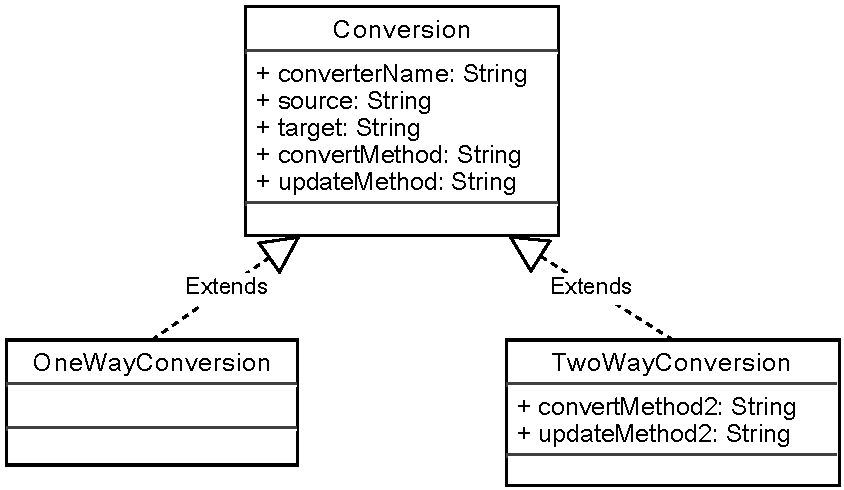
\includegraphics[width=0.6\textwidth]{chapteradapters/ConversionsUML.pdf}
\caption{The run-time \lstinln{Conversion} objects type hierarchy}
\label{fig:convclasses}
\end{figure}

From the conversion data two separate \lstinln{HashMap}s are generated; \lstinln{conversionMap} and \lstinln{sourceMap}.
The \lstinln{conversionMap} is a \lstinln{<String, Conversion>} mapping; the conversions are mapped with their unique ID.  
The \lstinln{sourceMap} is mapping from \lstinln{<Class<?>, ArrayList<String> >}, where \lstinln{Class} represents the source type of the conversion and the \lstinln{ArrayList<String>} is a list of unique IDs of conversion which convert from the source type declared as the key. 
The \lstinln{sourceMap} is constructed to avoid iterating over the whole \lstinln{conversionMap} while searching for an adapter. 

Conversion aspects register their source--target maps during initialization.
This is done by calling the \lstinln{register(String, Map)} method of the \lstinln{ZamkRuntime}. The \lstinln{String} value is the unique ID of the conversion and the \lstinln{Map} is the \lstinln{HashMap} or the \lstinln{BiHashMap} the aspect contains. 
The individual conversion maps are stored in a \lstinln{HashMap} called \lstinln{mapPerConversion}.
Even though the maps are declared and initialized in the conversion aspects, they are managed by the \lstinln{ZamkRuntime}.

\subsubsection{\zamk Conversion Requests}
The \zamk runtime is triggered by conversion requests. 
A conversion request passes on the source object and a desired target type, in return \zamk runtime provides an object which is initialized based on the values contained in the source object.
The conversion requests are communicated to \zamk with \lstinln{getConvertedValue(Object, Class<?>)} method, which is a static method of \lstinln{ZamkRuntime}.
The pseudo code for \lstinln{getConvertedValue} method is shown in Procedure~\ref{alg:value}. 
The step is to find the the suitable conversion for the given input by calling the \lstinln{findConversion} method (line~\ref{findconversion}). If this operation is successful, the unique ID of the found conversion is returned (the $uid$ variable). The details of the \lstinln{findConversion} method is discussed in section~\ref{sec:adapter:find}. 
Using $uid$ the source--target map for the conversion is retrieved from \lstinln{mapPerConversion} hash-map (line~\ref{getconversionmap}).
First we check if there is a source--target entry in the conversion map for the given source object, i.e. if the source object has been converted before using this conversion. 
If this is true, then the corresponding target object is retrieved and returned.
If the request triggers a new conversion, then the \lstinln{invokeConversion} method is called with the $uid$ and the source object to create a new target object. 
The new source--target pair is added to the $map$ and the target object is returned.


\begin{algorithm}
\caption{The \lstinln{getConveterdValue} method}\label{alg:value}
	\begin{algorithmic}[1]
		\Procedure{getConvertedValue}{$source, targetType$}
		\State $uid \gets findConversion(source, targetType)$ \label{findConversion}
		\State $map \gets mapPerConversion.get(uid)$ 
		\label{getconversionmap}
		\If{$source \in map$}
			\State return $map.get(source)$ \label{existingconversion}
		\Else
			\State $target \gets invokeConversion(uid, source)$ \label{newconversion}
			\State add $(source, target)$ pair to $map$ \label{addtomap}
			\State return $target$
		\EndIf
		\EndProcedure
	\end{algorithmic}
\end{algorithm}








\subsubsection{Finding the correct conversion}
\label{sec:adapter:find}
\begin{figure}[h]
\centering
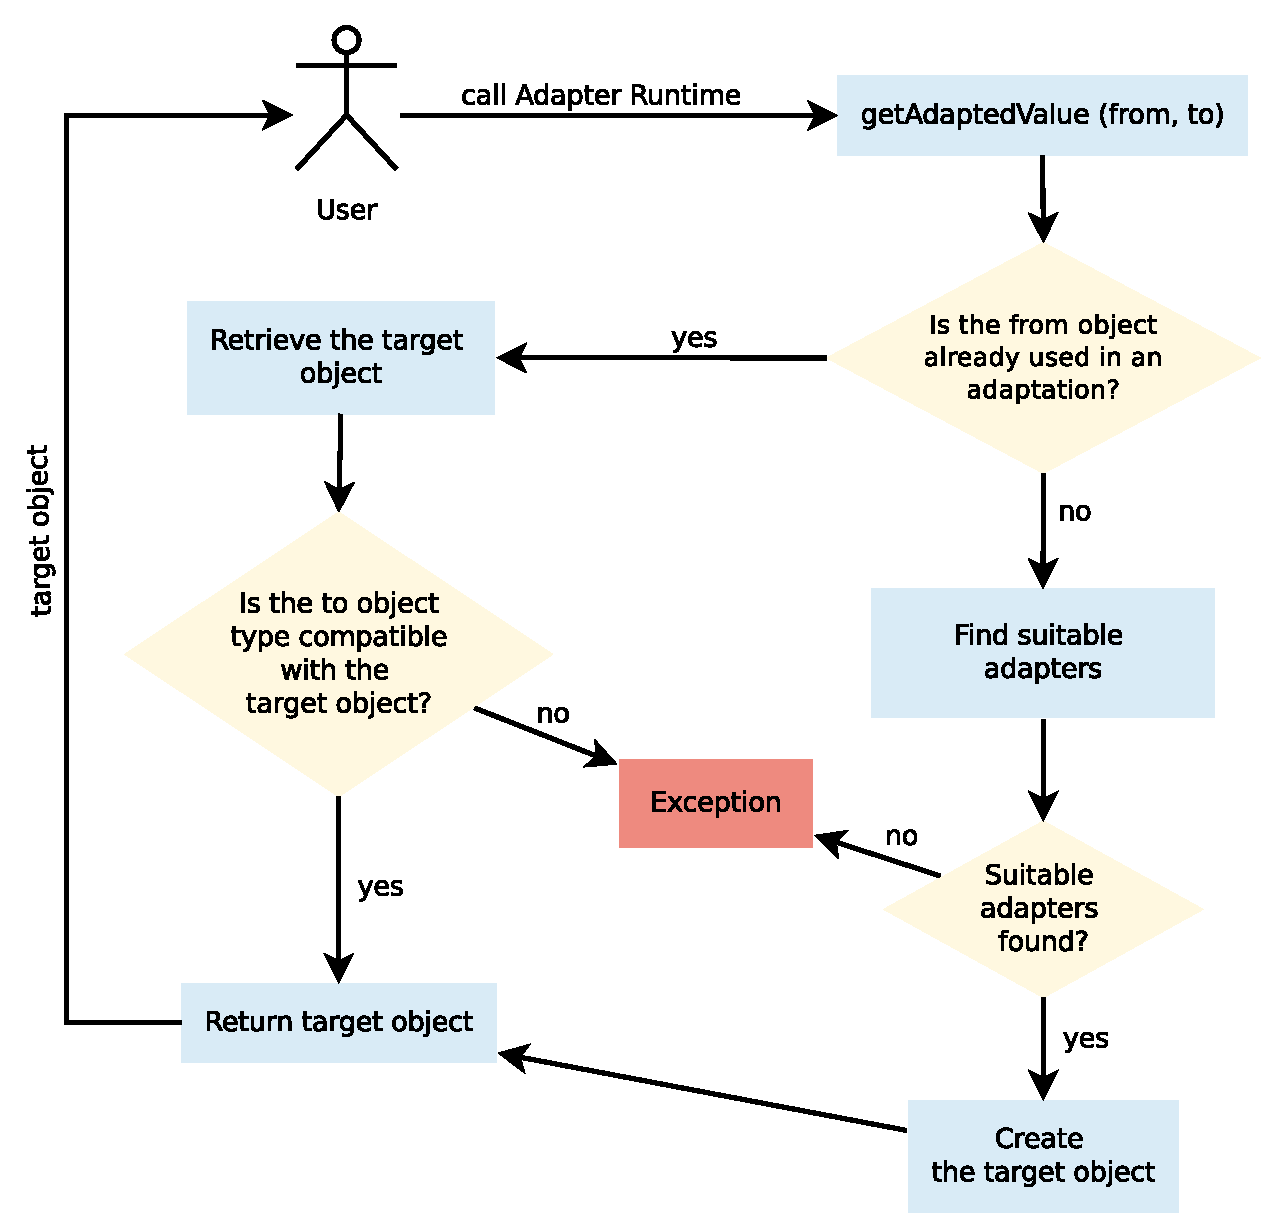
\includegraphics[width=0.8\textwidth]{chapteradapters/adapterruntimeflow.pdf}
\caption{The adaptation process flowchart}
\label{fig:arflowchart}
\end{figure}

\subsubsection{Target Object Retrieval}
\subsubsection{Object Synchronization}
\label{sec:adapter:sync}
\subsubsection{Fault Tolerance????}

\subsection{Using the Framework}
\subsubsection{Gluer DSL}
\subsubsection{Calling the run-time directly}

\section{Related Work}
\section{Conclusion}




% \paragraph{Adapter Runtime}
% Adapter runtime is responsible for applying correct adaptations and managing adaptee--target object pairs. Adapter runtime is an abstract aspect which provides the static method \lstinln{getAdaptedValue} as an entry point. This is a \emph{generic} method which takes the adaptee values and target's class as an argument. In figure~\ref{fig:arflowchart} we illustrate what happens when the user calls the \lstinln{getAdaptedValue}. 



% When the user requests an adaptation, i.e she provides an adaptee object and expects an object in return of a certain type (eXpected Target Type (XTT)), the first thing the frameworks checks is if the adaptee object is currently connected to a target object. There may be several such target objects hence the next step is to look if any of the target objects are type compatible with the user's XTT. Again, from these set of objects a subset may be type compatible, i.e may be assignable from the XTT. If this subset contains one object that's type is \emph{exactly} the same as the XTT then the \lstinln{getAdaptedValue} method returns this target object. If this list contains multiple object with exact XTT, then another resolution mechanism is applied, which will be explained later (\TODO{in section ?? Using aspect precedence for resolution}). 
% If there are no target object with the XTT, then the \emph{next most specific type} is assumed to be the XTT and the same steps are followed until a suitable target object is found. 
% The adapter runtime also provides the option to determine the depth of this search. The method can be called as \lstinln{getAdaptedValue(..,int)}, where the int value represents the level of the most distant acceptable type in the type hierarchy the XTT belongs to. If no object is found satisfying this criteria then a new target object is created using the appropriate adapter. 

% \begin{algorithm}
% \caption{Searching for target objects}\label{euclid}
% 	\begin{algorithmic}[1]
% 		\Procedure{SearchForTargetObject}{$adaptee, targetMap, XTT, depth$}
% 			\State $keySet \gets targetMap.keySet$
% 			\If{$keySet$ contains $adaptee$}
% 				\State $assocTarget \gets targetMap.get(adaptee)$
% 				\State $exactXTT \gets$ objects in $assocTarget$ with type exactly XTT 
% 				\If{$exactXTT.size > 1$}
% 					invoke precedence resolver
% 				\ElsIf{$exactXTT.size = 1$}
% 					\Return the first element of $exactXTT$
% 				\Else {$exactXTT$ is empty}
% 					\Repeat
% 					\State $closestXTT \gets$ objects in $assocTarget$ with subtype of XTT on $_depth$ level in type-hierarchy
% 					\If{target object is found in $closestXTT$}
% 						\Return object
% 					\EndIf
% 					\Until{$currentDepth <= depth$}
% 				\EndIf	
% 			\Else{}
% 				create target object
% 			\EndIf
			
% 		\EndProcedure
% 	\end{algorithmic}
% \end{algorithm}






% \section{Approach}
% We propose a new implementation for the adapter mechanism, which makes it possible to create adapters that are independent of the type hierarchies of the adapted components. This implementation strategy is enforced with a framework which takes a user defined adapter as an input and generates the adaptation specific aspect, which works with the \emph{adapter run-time} to keep the adaptee and the target objects synchronized. The adapter run-time is also responsible for creating and returning target objects given an adaptee object and a target type.
% An abstract overview of the framework is shown in Figure~\ref{fig:framework}.




% \paragraph{User-Defined Adapters}
% \TODO{The name of the annotations might change?}
